\documentclass[letterpaper]{article}
\usepackage[margin=1in]{geometry} % Sets page size and 1-inch margins
\usepackage[svgnames,dvipsnames]{xcolor}   % svgnames is a superset of dvipsnames

\usepackage{amsmath} % For math symbols like \land, \langle, \rangle, \to
\usepackage{array}   % For advanced column specifications
\usepackage{tabularx}% For tables with auto-expanding columns
\usepackage{tikz}
\usetikzlibrary{
    positioning,      % For placing nodes relative to each other (e.g., below=of)
    shapes.geometric, % For shapes like ellipses
    arrows.meta,      % For advanced arrow tips (e.g., Stealth)
    decorations.pathmorphing, % For snake/squiggly lines
    calc              % For coordinate calculations
}

% --- GLOBAL STYLE DEFINITIONS FOR DFD ---
\tikzset{
    % A shape for logical connectives
    connective_node/.style={
        rectangle, rounded corners=5pt, draw=black!80, fill=black!10, 
        inner sep=5pt, thick, align=center
    },
    % A shape for Introduction Rules
    intro_rule_node/.style={
        rectangle, rounded corners=5pt, draw=black!80, fill=Teal!20, 
        inner sep=5pt, thick, align=center
    },
    % A shape for Elimination Rules
    elim_rule_node/.style={
        rectangle, rounded corners=5pt, draw=black!80, fill=BurntOrange!20, 
        inner sep=5pt, thick, align=center
    },
    % A shape for abstract propositions
    proposition_node/.style={
        ellipse, draw=black!80, fill=Violet!15,
        inner sep=3pt, align=center
    },
    % A shape for concrete proof terms
    proof_node/.style={
        ellipse, draw=black!80, fill=Green!15,
        inner sep=3pt, align=center
    },
    % Arrow styles with color
    input_arrow/.style={-Stealth, solid, thick, draw=blue!70!black},
    output_arrow/.style={double, double distance=1.5pt, -Stealth, solid, thick, draw=ForestGreen!80!black},
    proves_arrow/.style={-Stealth, decorate, decoration={snake, segment length=6pt, amplitude=1pt}, thick, draw=orange!90!black}
}

% --- Define and measure boxes to get widths for tabularx ---
\newlength{\andheaderwidth}
\settowidth{\andheaderwidth}{\textbf{And} : Prop $\to$ Prop $\to$ Prop}
\newlength{\andintrofooterwidth}
\settowidth{\andintrofooterwidth}{\textbf{And.intro} : P $\to$ Q $\to$ P $\land$ Q}


\begin{document}

\begin{figure}[h!]
\centering
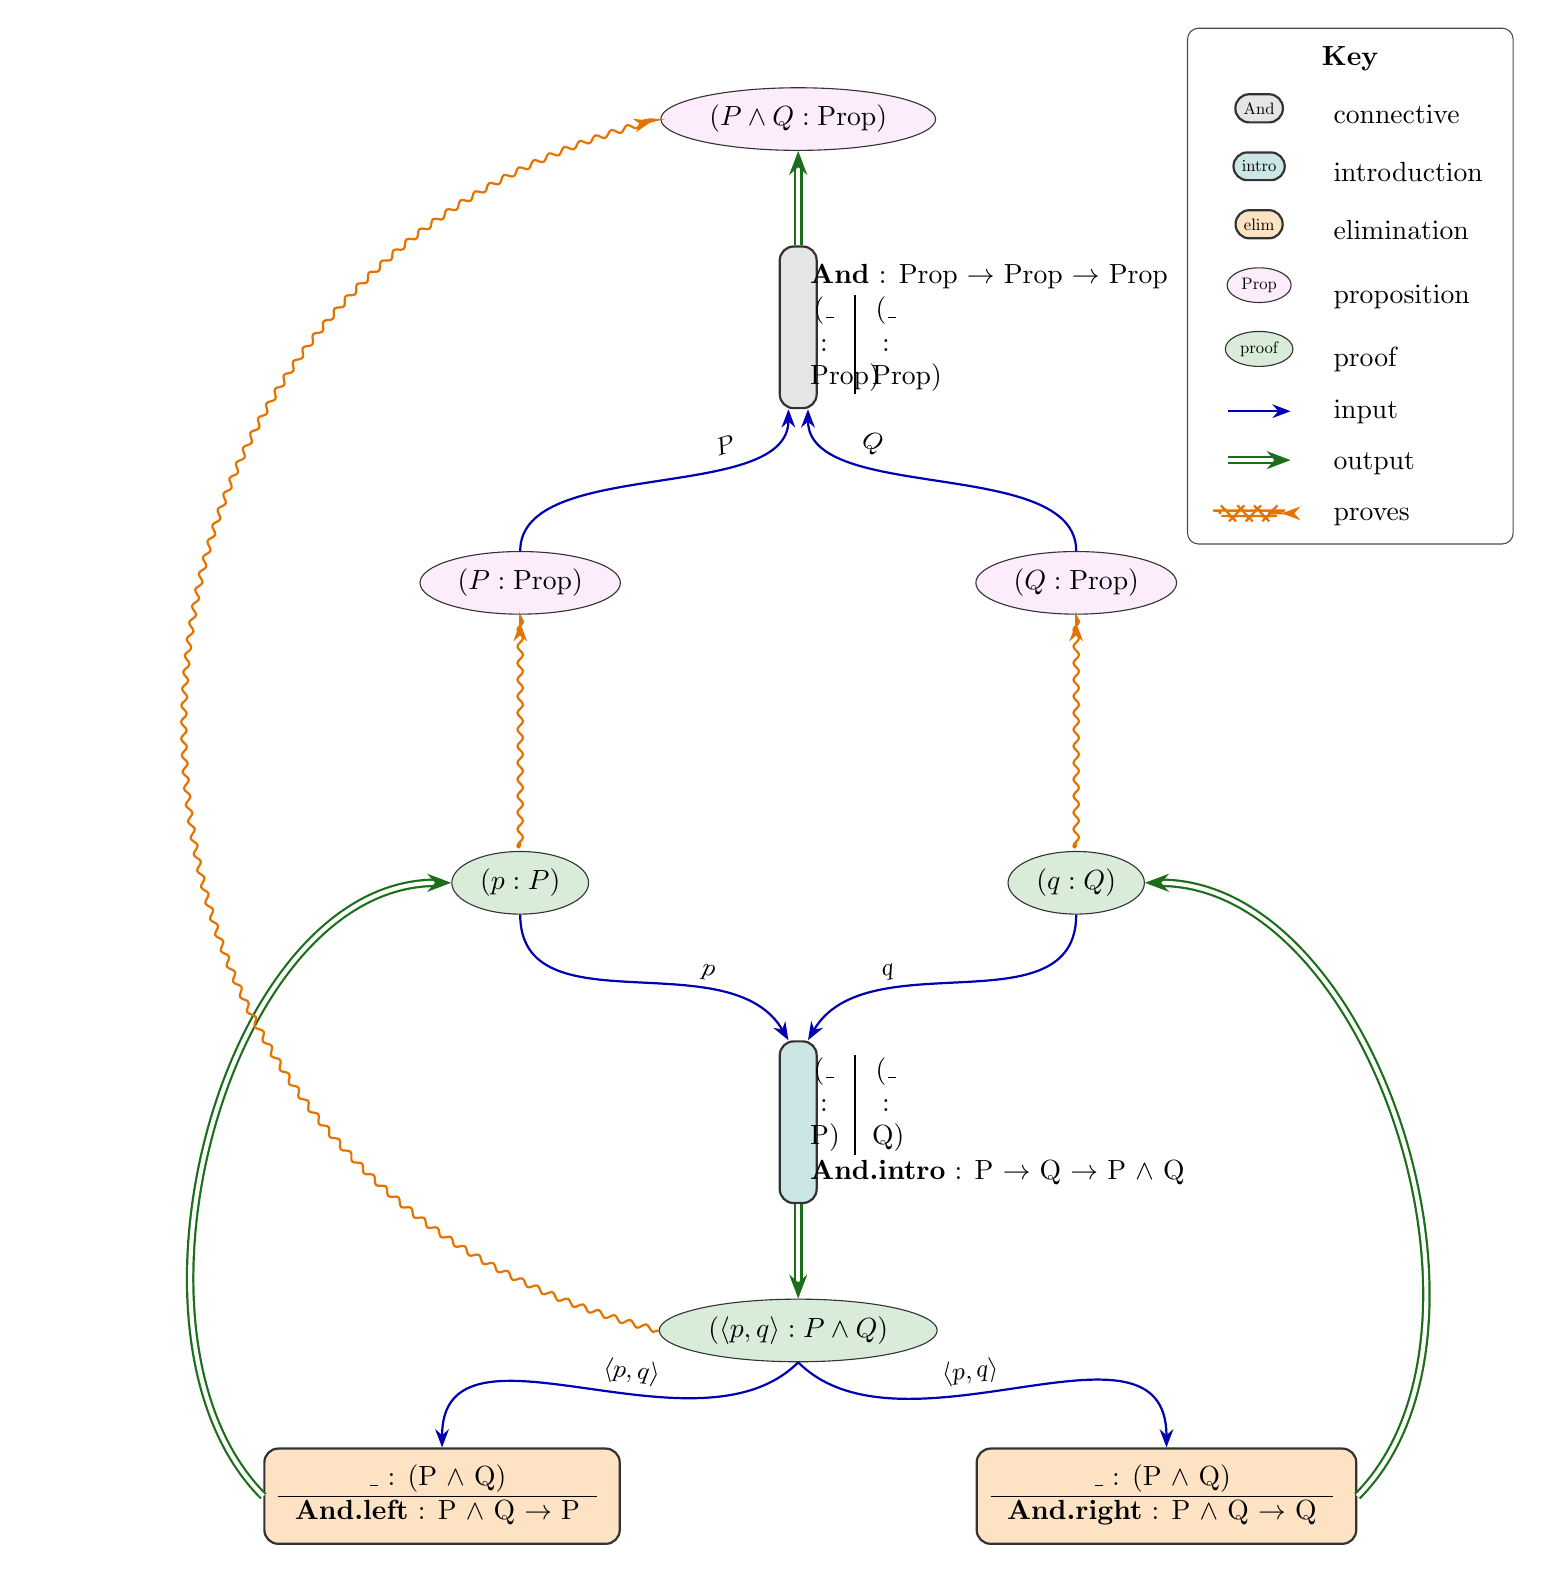
\begin{tikzpicture}[node distance=2.2cm and 2.5cm]

% --- AESTHETIC REFINEMENT: Define a single variable for the main arc's width ---
\newcommand{\outset}{8.0} % Using \newcommand for safety

% --- NODE DEFINITIONS WITH FINAL STYLES ---

% Top layers of proposition nodes
\node[proposition_node] (P_prop) {$(P : \text{Prop})$};
\node[proposition_node] (Q_prop) [right=4.5cm of P_prop] {$(Q : \text{Prop})$};

% Top-level Connective node
\node[connective_node, above=1.8cm of $(P_prop.north)!.5!(Q_prop.north)$] (and_box) {
    \begin{tabularx}{\andheaderwidth}{>{\centering\arraybackslash}X|>{\centering\arraybackslash}X}
        \multicolumn{2}{c}{\textbf{And} : Prop $\to$ Prop $\to$ Prop} \\ \hline
        (\_ : Prop) & (\_ : Prop)
    \end{tabularx}
};

\node[proposition_node] (P_and_Q_prop) [above=1.2cm of and_box] {$(P \land Q : \text{Prop})$};

% Middle layers of proof nodes
\node[proof_node] (p_P) [below=3cm of P_prop] {$(p : P)$};
\node[proof_node] (q_Q) [below=3cm of Q_prop] {$(q : Q)$};

% Central Introduction Rule node
\node[intro_rule_node, below=2cm of $(p_P)!.5!(q_Q)$] (and_intro) {
    \begin{tabularx}{\andintrofooterwidth}{>{\centering\arraybackslash}X|>{\centering\arraybackslash}X}
    (\_ : P) & (\_ : Q) \\ \hline
    \multicolumn{2}{c}{\textbf{And.intro} : P $\to$ Q $\to$ P $\land$ Q}
    \end{tabularx}
};

\node[proof_node] (pq_pair) [below=1.2cm of and_intro] {$(\langle p, q \rangle : P \land Q)$};

% Bottom layer of Elimination Rule nodes
\node[elim_rule_node, below left=1.2cm and 1cm of pq_pair] (and_left) {
    \begin{tabular}{c}
    \_ : (P $\land$ Q) \\ \hline
    \textbf{And.left} : P $\land$ Q $\to$ P
    \end{tabular}
};

\node[elim_rule_node, below right=1.2cm and 1cm of pq_pair] (and_right) {
    \begin{tabular}{c}
    \_ : (P $\land$ Q) \\ \hline
    \textbf{And.right} : P $\land$ Q $\to$ Q
    \end{tabular}
};


% --- BEAUTIFUL EDGE ROUTING ---
\draw[output_arrow] (and_box) -> (P_and_Q_prop);

% --- AESTHETIC REFINEMENT: Use a smaller font size for arrow labels ---
\draw[input_arrow] (P_prop.north) to[out=90, in=-90, looseness=0.8] node[pos=0.7, sloped, above, font=\small] {$P$} ($(and_box.south west)!.5!(and_box.south)$);
\draw[input_arrow] (Q_prop.north) to[out=90, in=-90, looseness=0.8] node[pos=0.7, sloped, above, font=\small] {$Q$} ($(and_box.south)!.5!(and_box.south east)$);

\draw[input_arrow] (p_P.south) to[out=-90, in=120] node[pos=0.7, sloped, above, font=\small] {$p$} ($(and_intro.north west)!.5!(and_intro.north)$);
\draw[input_arrow] (q_Q.south) to[out=-90, in=60] node[pos=0.7, sloped, above, font=\small] {$q$} ($(and_intro.north)!.5!(and_intro.north east)$);

\draw[output_arrow] (and_intro) -> (pq_pair);

% Graceful arcs for input arrows from the bottom
\draw[input_arrow] (pq_pair.south) to[out=-135, in=90] node[pos=0.4, sloped, above, font=\small] {$\langle p, q \rangle$} (and_left.north);
\draw[input_arrow] (pq_pair.south) to[out=-45, in=90] node[pos=0.4, sloped, above, font=\small] {$\langle p, q \rangle$} (and_right.north);

% Output arrows from the SIDES of the left/right boxes.
\draw[output_arrow] (and_left.west) to[out=135, in=180, looseness=0.9] (p_P.west);
\draw[output_arrow] (and_right.east) to[out=45, in=0, looseness=0.9] (q_Q.east);

% Type/proves arrows are now shortened.
\draw[proves_arrow, shorten <=3pt, shorten >=3pt] (p_P) -> (P_prop);
\draw[proves_arrow, shorten <=3pt, shorten >=3pt] (q_Q) -> (Q_prop);

% Main "proves" arc, using the \outset variable for easy adjustment.
\coordinate (c1) at ($(pq_pair.west)+(-\outset,2)$);
\coordinate (c2) at ($(P_and_Q_prop.west)+(-\outset,-2)$);
\draw[proves_arrow, shorten >=3pt] (pq_pair.west) .. controls (c1) and (c2) .. (P_and_Q_prop.west);


% --- FINAL LEGEND ---
\node (legend) [draw=black!70, rounded corners, inner sep=5pt, above right=0.2cm and 0.5cm of Q_prop] {
    % --- AESTHETIC REFINEMENT: Use specified lengths for consistent vertical spacing ---
    \begin{tabular}{cl}
    \multicolumn{2}{c}{\textbf{Key}} \\[1.5ex]
    \tikz{\node[connective_node, scale=0.6] {And};} & connective \\[1.5ex]
    \tikz{\node[intro_rule_node, scale=0.6] {intro};} & introduction \\[1.5ex]
    \tikz{\node[elim_rule_node, scale=0.6] {elim};} & elimination \\[1.5ex]
    \tikz{\node[proposition_node, scale=0.6] {Prop};} & proposition \\[1.5ex]
    \tikz{\node[proof_node, scale=0.6] {proof};} & proof \\[1.5ex]
    \tikz{\draw[input_arrow] (0,0.1) -- (0.8,0.1);} & input \\[1.5ex]
    \tikz{\draw[output_arrow] (0,0.1) -- (0.8,0.1);} & output \\[1.5ex]
    \tikz{\draw[proves_arrow] (0,0.1) -- (0.8,0.1);} & proves \\
    \end{tabular}
};

\end{tikzpicture}
% --- CAPTION REFINEMENT: Corrected typos and grammar ---
\caption{The algebra of logical conjunction. The And function takes two propositions, call them $P$ and $Q$, 
and yields the proposition that is their logical conjunction, $P \land Q$. The $And.intro$ function takes
two proofs, $p$ of $P$ and $q$ of $Q$, and returns a proof, $\langle p, q \rangle$, of their conjunction. The $And.left$
function takes a proof, $\langle p, q \rangle$ of $P \land Q$, and returns the proof $(p : P)$, while $And.right$ returns 
the proof $(q : Q)$. All of these proof handling functions implicitly take the types P and Q themselves as 
implicit arguments. They are typically not provided explicitly when these functions are applied to their 
arguments, but are inferred automatically from the types of these arguments; and we've elided them from
this diagram.}
\label{fig:tikz_diagram_definitive}
\end{figure}

\end{document}